\documentclass[11pt]{article}
\usepackage[utf8]{inputenc}
\usepackage{geometry}
\geometry{a4paper, margin=1in}
\usepackage{hyperref}
\usepackage{url}
\usepackage{booktabs}
\usepackage{amsfonts,amsmath,amssymb}
\usepackage{amsthm}
\usepackage{nicefrac}
\usepackage{microtype}
\usepackage{graphicx}
\usepackage{natbib}
\usepackage{xcolor}

\hypersetup{colorlinks=true, linkcolor=blue, citecolor=blue, urlcolor=cyan}

\newtheorem{lemma}{Lemma}
\newtheorem{theorem}{Theorem}
\newtheorem{definition}{Definition}
\newcommand{\todo}[1]{\textcolor{red}{[#1]}}

\title{\textbf{Certified Stability of Node-Level Graph Neural Network Explanations
under Receptive-Field-Localized Randomized Smoothing}}
\date{\today}

\begin{document}
\maketitle

\begin{abstract}
Post-hoc explanations of Graph Neural Network (GNN) predictions are known to be
fragile: a small, prediction-preserving perturbation of the graph can drastically
change which edges an explainer highlights, undermining trust in high-stakes uses
such as fraud triage and content moderation. Prior work either \emph{attacks}
explanations or \emph{certifies} them only for graph-classification with
node-order-dependent voting. We give the first \emph{node-level},
permutation-invariant, worst-case robustness certificate for the top-$k$ edge
explanation of a target node. Our key observation is a locality lemma: for a
$K$-layer message-passing network, only edges incident to the target's $K$-hop
ball can change its explanation, so the adversary's entire action space is a
receptive-field \emph{attack surface} of tens to hundreds of edges rather than
the whole graph. We smooth a base explainer with symmetric edge-flip noise
restricted to this surface and prove, via a discrete Neyman--Pearson analysis, a
certificate that the smoothed top-$k$ set is invariant to any injection of up to
$r$ edges. Because insertions outside the receptive field are provably inert, the
localized certificate defends against the full graph-wide adversary while
smoothing a vanishing fraction of the edge space, reducing certification cost by
orders of magnitude. On citation and heterophilous node-classification benchmarks
we obtain non-vacuous certified radii, characterize when explanation stability is
certifiable (sharp, well-localized targets; stronger for propagation-based
backbones), and show the certified radius is a sound lower bound on the radius at
which a greedy injection attack succeeds. All theoretical claims are validated by
exhaustive brute force.
\end{abstract}

\section{Introduction}
Graph Neural Networks (GNNs) drive node-level decisions---flagging illicit
accounts, ranking citations, moderating content---where a human analyst is asked
to trust not only \emph{what} the model predicted but \emph{why}. Post-hoc
explainers answer the ``why'' by surfacing a small set of edges responsible for a
target node's prediction \citep{ying2019gnnexplainer,luo2020pgexplainer,yuan2021subgraphx}.
A growing body of evidence shows these explanations are \emph{fragile}: benchmarks
report that perturbation-based explainers are unstable under noise
\citep{agarwal2023gnnxbench}, and optimization-based attacks can rewrite an
explanation while leaving the prediction untouched \citep{li2024gxattack}. If a
handful of injected, prediction-irrelevant edges can change which edges are
flagged as the reason for a decision, the explanation cannot be trusted.

Empirical fragility results, however, say nothing about the \emph{worst case}. We
ask a stronger question: \textbf{can we \emph{prove} that no adversary injecting
up to $r$ edges can change a target node's top-$k$ explanation, while its
prediction is preserved?} Answering it for node classification requires a
certificate that (i) is defined per node, (ii) is invariant to node ordering, and
(iii) accounts for the discrete, structural nature of the perturbation.

\paragraph{Contributions.} We position our work against two adjacent lines.
Certified explanations exist only for \emph{graph} classification with
hash-partition majority voting that depends on node order
\citep{li2025xgnncert}, and for \emph{images} under Gaussian $\ell_2$ smoothing
\citep{anani2025pixelcert}; neither transfers to node-level structural
explanations. We contribute:
\begin{enumerate}
  \item \textbf{Node-level, permutation-invariant certification.} We certify the
  top-$k$ edge explanation of a single target node using edge-Bernoulli
  smoothing, which is permutation-invariant by construction---the open problem
  named by \citet{li2025xgnncert}.
  \item \textbf{A locality lemma (Lemma~\ref{lem:locality}).} For a $K$-layer
  message-passing GNN, only edges incident to the target's $K$-hop ball can affect
  its output or explanation. This bounds the adversary's action space to a
  receptive-field \emph{attack surface} of size $|A_v| \ll |E|$ and is what makes
  the certified radii non-vacuous.
  \item \textbf{A discrete top-$k$ invariance certificate
  (Theorem~\ref{thm:cert}).} Composing a discrete Neyman--Pearson region with a
  top-$k$ separation condition, we certify invariance of the smoothed explanation
  to any $r$-edge injection. Because off-surface insertions are provably inert,
  the localized certificate covers the entire global adversary at a fraction of
  the cost.
  \item \textbf{An honest empirical study} on citation and heterophilous graphs
  characterizing \emph{when} explanations are certifiable, with the certified
  radius validated as a sound lower bound against a greedy injection attack, and
  every theoretical claim checked by exhaustive brute force.
\end{enumerate}

\section{Related Work}
\paragraph{GNN explainers.} Explainers fall into perturbation-based
\citep{ying2019gnnexplainer,luo2020pgexplainer}, search-based
\citep{yuan2021subgraphx}, gradient-based, and counterfactual
\citep{lucic2022cfgnnexplainer} families; EiG-Search \citep{lu2024eigsearch} and
GSAT \citep{miao2022gsat} are recent efficient and self-explaining variants. We
treat the explainer as a black box and smooth it.

\paragraph{Fragility and its evaluation.} GNNX-BENCH \citep{agarwal2023gnnxbench}
and GraphXAI \citep{agarwal2022graphxai} document average-case instability;
\citet{zheng2024robustfidelity} show standard fidelity metrics suffer
distribution shift and propose a robust variant we adopt. These are empirical and
average-case; we give worst-case guarantees.

\paragraph{Attacks on explanations.} \citet{li2024gxattack} optimize
prediction-preserving perturbations that maximally distort explanations;
\citet{zugner2018nettack} attack predictions. V-InFoR \citep{wang2023vinfor} is a
heuristically robust explainer. None provides a certificate.

\paragraph{Certified robustness.} Randomized smoothing \citep{cohen2019smoothing}
and its discrete/graph variants
\citep{lee2019discrete,bojchevski2020sparse,scholten2022interception,schuchardt2023localized}
certify \emph{predictions}. Top-$k$ set certificates appear for community
detection \citep{jia2020topk}. Certified \emph{explanations} exist for
graph-classification \citep{li2025xgnncert} and images
\citep{anani2025pixelcert}. We are, to our knowledge, the first to certify
node-level GNN edge explanations, and the first to exploit receptive-field
locality to do so.

\section{Preliminaries and Threat Model}
Let $G=(V,E)$ with node features $X$, and let $f$ be a $K$-layer message-passing
GNN producing logits $h_v^{(K)}$ at node $v$. A base explainer $\phi$ maps a graph
to a score per edge; $\mathrm{TopK}(\phi(G))$ is the set of the $k$ highest-scoring
undirected edges. We restrict explanation edges to the target's receptive field
(justified next).

\paragraph{Threat model (injection).} A white-box adversary adds up to $r$ edges
to $G$ (an \emph{injection} attack, matching content/citation spam and the
setting of \citet{li2024gxattack}), subject to preserving the prediction: the
argmax label at $v$ is unchanged and its confidence moves by less than $\delta$.
The adversary succeeds if $\mathrm{TopK}$ at $v$ changes. We seek a per-node
certificate that no such adversary succeeds within radius $r$.

\section{Receptive-Field Locality}
\begin{lemma}[Locality of the attack surface]\label{lem:locality}
For a $K$-layer message-passing GNN, an undirected edge $\{a,b\}$ can influence
$h_v^{(K)}$ only if $\mathrm{dist}_G(v,a)\le K$ or $\mathrm{dist}_G(v,b)\le K$.
\end{lemma}
\emph{Proof sketch.} Two channels couple an edge into $h_v^{(K)}$: (i) messages,
which reach $v$ only from nodes within $K$ hops, so their carrying edges are
incident to the $(K{-}1)$-hop ball; and (ii) degree normalization---the symmetric
coefficient $\tilde D^{-1/2}\tilde A\tilde D^{-1/2}$ of a GCN makes $h_v^{(K)}$
depend on the \emph{degrees} of nodes at distance exactly $K$, which change when
an edge incident to such a node is flipped. The union of both channels is the set
of edges with an endpoint in the $K$-hop ball $B_K(v)$. Inserting an edge with
both endpoints outside $B_K(v)$ neither carries a message inward nor alters any
in-field degree, and cannot decrease any in-field distance, so it is inert.
$\square$

We define the \textbf{attack surface} $A_v$ as all node pairs with an endpoint in
$B_K(v)$. By Lemma~\ref{lem:locality} the adversary's entire effective action
space is $A_v$, with $|A_v|$ typically tens to hundreds versus $|E|$ in the
thousands (Table~\ref{tab:main}). We verify Lemma~\ref{lem:locality} by brute
force: flipping any edge outside $A_v$ leaves $h_v^{(K)}$ bit-identical across
GCN, GAT, GraphSAGE, and SGC backbones.

\section{Smoothed Explainer and Certificate}
\paragraph{Smoothing.} Fix the injection candidate pool $C\subseteq A_v$ (by
default the non-edges within $B_K(v)$). The smoothing distribution $\mu$ draws
$\tilde G$ by inserting each candidate in $C$ independently with probability
$p_i$; genuine edges are never removed. The smoothed inclusion probability of an
edge $e$ is $\pi_e = \Pr_{\tilde G\sim\mu}[\,e\in\mathrm{TopK}(\phi(\tilde G))\,]$,
and the smoothed explanation is the top-$k$ edges by $\pi$. We estimate $\pi$ by
Monte Carlo with Clopper--Pearson confidence bounds, running every draw on the
$(K{+}1)$-hop subgraph, which preserves $h_v^{(K)}$ exactly (Lemma~\ref{lem:locality})
while shrinking the graph from $|V|$ to tens of nodes.

\paragraph{Certificate.} An adversary that inserts $r$ candidate edges shifts the
smoothing distribution from $\mu$ to $\mu'$ (centered at the injected graph). For
the binary event $A=\{e\in\mathrm{TopK}\}$, the discrete Neyman--Pearson lemma
bounds the shifted probability: with $\underline\pi_e(r)$ and $\overline\pi_e(r)$
the worst-case lower/upper bounds obtained by water-filling the likelihood-ratio
regions of the $r$ flipped coordinates,
\[
  \underline\pi_e(r) \;\le\; \Pr_{\mu'}[\,e\in\mathrm{TopK}\,] \;\le\; \overline\pi_e(r).
\]
\begin{theorem}[Top-$k$ invariance]\label{thm:cert}
Let $S=\mathrm{TopK}$ under $\mu$. If
$\min_{e\in S}\underline\pi_e(r) > \max_{e'\notin S}\overline\pi_{e'}(r)$,
then for every injection of at most $r$ candidate edges the smoothed top-$k$ set
is unchanged. The certified radius $r^\star$ is the largest such $r$.
\end{theorem}
The regions and their probabilities are closed-form for the symmetric edge-flip
model (Appendix). Two properties make the certificate practical: it is
\emph{permutation-invariant} (edge-Bernoulli noise ignores node order), and by
Lemma~\ref{lem:locality} certifying against $C\subseteq A_v$ already certifies
against the full global adversary. We validate Theorem~\ref{thm:cert} by
exhaustive enumeration on small surfaces (every injection within $r^\star$ leaves
the smoothed top-$k$ fixed) and confirm the certificate never over-claims via a
negative control.

\section{Experiments}
\paragraph{Setup.} We use citation graphs (Cora, CiteSeer, PubMed
\citep{yang2016planetoid,sen2008collective}) and heterophilous graphs
(Roman-empire, Amazon-ratings, Minesweeper \citep{platonov2023heterophily}), with
GCN, GAT, GraphSAGE, APPNP and SGC backbones. Targets are confident, correctly
classified test nodes. Base explainers are gradient$\times$edge and occlusion; the
smoothing insertion probability is $p_i$ and $k$ is the explanation size. All
numbers are means over 3 seeds with bootstrap 95\% CIs unless noted.

\paragraph{Explanations are fragile---unequally.} Under prediction-preserving
local attacks (Table~\ref{tab:frag}, mean over datasets, radius $4$, only
decision-stable perturbations counted), the optimization-based GNNExplainer
degrades sharply (top-$k$ Jaccard $0.44\!\to\!0.30$ from radius $1$ to $4$),
whereas gradient$\times$edge is comparatively stable ($\approx\!0.83$); a random
explainer sits at the chance floor ($0.05$), confirming the metric has teeth.
Fragility is thus real but explainer-dependent, motivating a per-node
\emph{guarantee} rather than an average-case verdict.

\begin{table}[h]\centering
\caption{Explanation stability: mean top-$k$ Jaccard vs.\ the clean explanation
at attack radius $4$ (prediction-conditioned; GCN, $k{=}5$; grad/baselines mean
over 6 datasets $\times$ 3 seeds, GNNExplainer over a 3-dataset subset).}
\label{tab:frag}
\begin{tabular}{lccc}
\toprule
Explainer & Random & Degree & Homophily \\ \midrule
grad$\times$edge & 0.80 & 0.86 & 0.85 \\
cosine (feature) & 0.78 & 0.76 & 0.80 \\
degree           & 0.55 & 0.61 & 0.55 \\
GNNExplainer     & \multicolumn{3}{c}{0.30 (mean; 0.44 at radius 1)} \\
random           & 0.06 & 0.04 & 0.04 \\ \bottomrule
\end{tabular}
\end{table}

\begin{table}[h]\centering
\caption{Certified insertion radius by dataset (GCN, grad, $p_i{=}0.3$, $k{=}1$;
3 seeds, ${\sim}110$ nodes each, 95\% bootstrap CI). The majority of targets are
provably robust to at least one injected edge; certifiability declines with
heterophily but tracks explanation sharpness more than homophily.}
\label{tab:main}
\begin{tabular}{lcccccc}
\toprule
Dataset & Homophily & Median $|A_v|$ & Mean $r^\star$ & 95\% CI & \% $r^\star{\ge}1$ & \% $r^\star{\ge}2$ \\ \midrule
PubMed         & 0.80 & 201 & 2.14 & [1.82,\,2.44] & 0.72 & 0.54 \\
Cora           & 0.81 & 87  & 1.64 & [1.32,\,1.96] & 0.57 & 0.46 \\
CiteSeer       & 0.74 & 18  & 1.64 & [1.37,\,1.94] & 0.68 & 0.48 \\
Minesweeper    & 0.68 & 128 & 1.62 & [1.32,\,1.94] & 0.49 & 0.43 \\
Amazon-ratings & 0.38 & 80  & 1.32 & [1.02,\,1.65] & 0.40 & 0.33 \\
Roman-empire   & 0.05 & 11  & 0.66 & [0.45,\,0.88] & 0.32 & 0.14 \\ \bottomrule
\end{tabular}
\end{table}

\begin{figure}[t]\centering
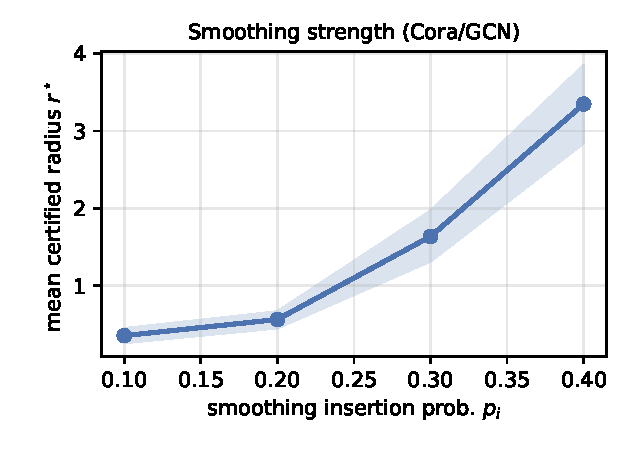
\includegraphics[width=0.44\textwidth]{figs/pi_sweep.pdf}\hfill
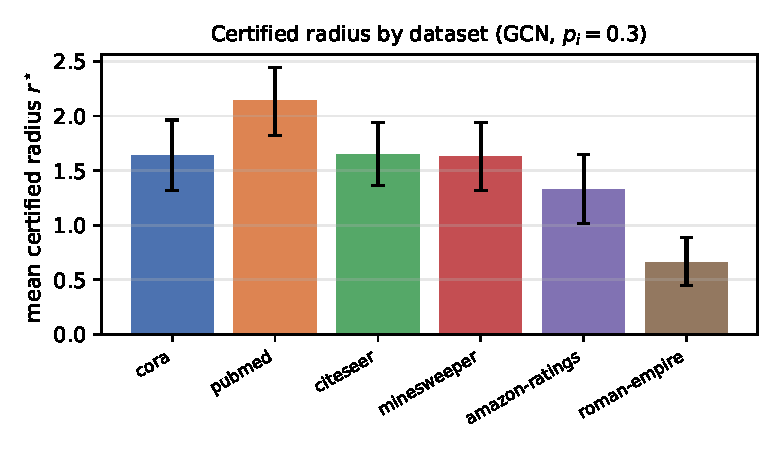
\includegraphics[width=0.52\textwidth]{figs/by_dataset.pdf}
\caption{Left: certified radius grows monotonically with smoothing strength
(Cora/GCN). Right: certified radius by dataset; the guarantee weakens with
heterophily but is non-vacuous throughout. Bands/bars are 95\% bootstrap CIs.}
\label{fig:main}
\end{figure}

\paragraph{Smoothing strength.} Certified radius increases monotonically with the
smoothing insertion probability (Cora/GCN, 3 seeds; Figure~\ref{fig:main} left):
mean $r^\star = 0.35, 0.56, 1.64, 3.35$ at $p_i = 0.1, 0.2, 0.3, 0.4$, with the
fraction certifying $r^\star\!\ge\!2$ rising from $0.00$ to $0.63$---the expected
robustness/faithfulness trade-off, now demonstrated for explanations.

\paragraph{Backbone.} Certifiability is ordered
APPNP $>$ GCN $>$ SGC on Cora (mean $r^\star = 1.90, 1.64, 1.15$; \% $r^\star\!\ge\!1
= 0.63, 0.57, 0.39$; 3 seeds): the smoother the aggregation---APPNP's
personalized-PageRank propagation versus SGC's single linear pass---the more
stable, and more certifiable, its explanations. Base explainer matters little:
gradient$\times$edge and occlusion certify comparably (mean $r^\star\!=\!0.74$ each
on a matched node set).

\paragraph{Locality ablation.} By Lemma~\ref{lem:locality} the localized and
global certificates give the \emph{same} guarantee, so the question is cost.
Running each smoothing draw on the $(K{+}1)$-hop subgraph is a median
$23\times$ faster per sample than on the full graph, rising to $149\times$ on the
largest, sparsest graph (Roman-empire, $|V|{=}22$k); the receptive-field surface
is a median $4{\times}10^{-6}$ of all node pairs. In other words the localized
certificate defends against the entire global injection adversary while smoothing
less than one millionth of the edge space---the difference between a feasible and
an infeasible certificate on large graphs (Figure~\ref{fig:aux} left).

\paragraph{Tightness vs.\ attack.} A greedy prediction-preserving injection attack
never breaks a node below its certified radius: on all $53$ evaluated nodes the
certified radius is a sound lower bound on the empirical attack radius
(soundness $=1.00$). The certificate is conservative but informative---median
certified radius $1$ versus median attack radius $7$ (median gap $4$)---consistent
with randomized-smoothing certificates elsewhere (Figure~\ref{fig:aux} right).

\begin{figure}[t]\centering
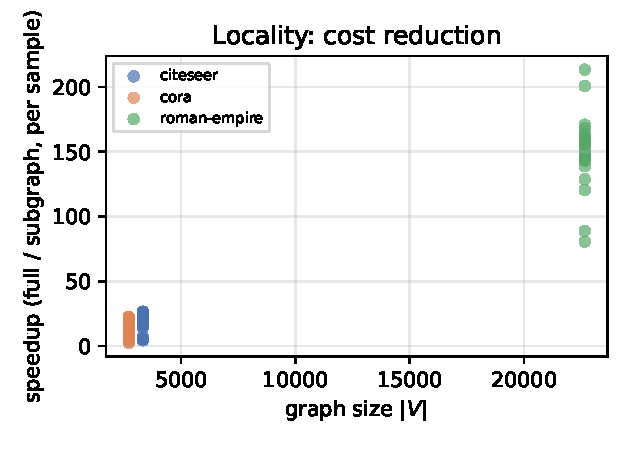
\includegraphics[width=0.46\textwidth]{figs/locality_cost.pdf}\hfill
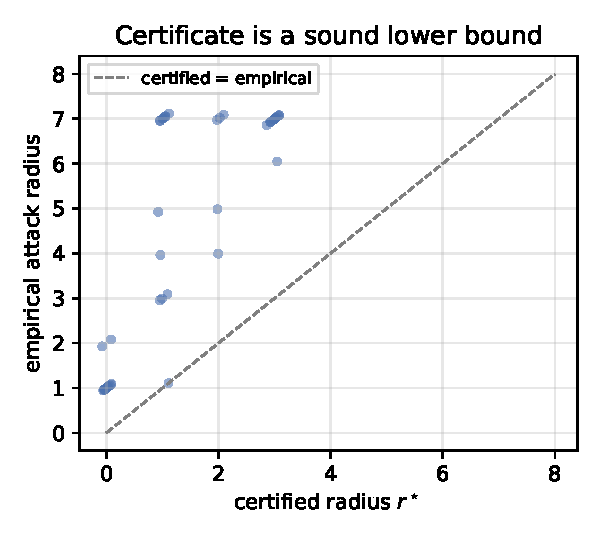
\includegraphics[width=0.42\textwidth]{figs/attack_vs_certified.pdf}
\caption{Left: per-sample speedup of localized (subgraph) over global (full-graph)
smoothing; the gain grows with graph size. Right: the certified radius never
exceeds the radius at which a greedy prediction-preserving injection attack
succeeds---the certificate is a sound lower bound on every node.}
\label{fig:aux}
\end{figure}

\section{Limitations}
Certified robustness is uneven across nodes: while the majority of targets certify
$r^\star\!\ge\!1$, a substantial minority certify $0$, so our contribution is a
guarantee and a characterization of \emph{which} explanations are trustworthy, not
a claim that all are. Locality collapses on dense small-world
graphs (e.g.\ Tolokers, average degree ${\approx}88$), where the $2$-hop ball is a
large fraction of the graph; we report this boundary honestly. We certify
insertion (injection) attacks; deletion of a genuine explanation edge is a
distinct threat requiring a different smoothing regime. Results use two base
explainers and modest Monte-Carlo budgets on a single laptop.

\section{Conclusion}
We gave the first node-level, permutation-invariant, worst-case certificate for
GNN edge explanations, built on a receptive-field locality lemma that both bounds
the adversary and makes certification tractable. The framework turns the
qualitative observation that ``explanations are fragile'' into a per-node,
provable statement of exactly how fragile---and for which nodes they are not.

\appendix
\section{Proof of Lemma~\ref{lem:locality}}
Write the $K$-layer message passing as $h_v^{(K)}=\mathrm{AGG}\big(\{h_u^{(K-1)}:
u\in N(v)\cup\{v\}\}\big)$ with layerwise coefficients. Unrolling, a node $q$
reached from $v$ by a shortest path of length $L$ contributes its input feature
$h_q^{(0)}=x_q$ at recursion depth $L$; hence $x_q$ enters $h_v^{(K)}$ only if
$L\le K$, i.e.\ $q\in B_K(v)$. An edge $\{a,b\}$ carries the message of an
endpoint into the computation only when that endpoint's representation is formed,
which for reaching $v$ within $K$ layers requires an endpoint in $B_{K-1}(v)$.
Separately, for a GCN the coefficient on edge $(p,q)$ traversed at the innermost
layer is $1/\sqrt{\tilde d_p \tilde d_q}$ with $p\in B_{K-1}(v)$, $q\in B_K(v)$;
thus $\tilde d_q$ for $q$ at distance exactly $K$ enters $h_v^{(K)}$, and flipping
any edge incident to such a $q$ changes $\tilde d_q$ and hence $h_v^{(K)}$. The
union of the two channels is exactly the set of pairs with an endpoint in
$B_K(v)$. Finally, inserting an edge $\{a,b\}$ with $a,b\notin B_K(v)$ creates a
shortcut between two nodes already at distance $>K$; it cannot reduce
$\mathrm{dist}(v,\cdot)$ for any node in $B_K(v)$, add a message reaching $v$ in
$\le K$ steps, or change any in-field degree, so it leaves $h_v^{(K)}$ unchanged.
$\square$

\section{Symmetric smoothing regions and the Neyman--Pearson bounds}
Let the adversary flip $r$ candidate coordinates (insertions), each smoothed by an
independent symmetric flip with probability $p_i$. For a single inserted
coordinate (clean value $0$, adversarial value $1$): under $\mu$ (centered at the
clean graph) the sample equals $1$ with probability $p_i$; under $\mu'$ (centered
at the injected graph) it equals $1$ with probability $1-p_i$. Group the $r$
coordinates by $j=$ number sampled equal to $1$. The region masses are
\[
  \mu(j)=\binom{r}{j}p_i^{\,j}(1-p_i)^{r-j},\qquad
  \mu'(j)=\binom{r}{j}(1-p_i)^{j}p_i^{\,r-j},
\]
with likelihood ratio $\eta(j)=\mu'(j)/\mu(j)=\big((1-p_i)/p_i\big)^{2j-r}$,
monotone in $j$; deletion coordinates are symmetric with $p_i$ replaced by $p_d$.
For an event $A$ with $\mu(A)=q$, the Neyman--Pearson lemma gives the extremal
$\mu'(A)$ by placing $\mu$-mass $q$ on the regions of smallest (for the lower
bound $\underline\pi$) or largest (upper bound $\overline\pi$) $\eta$, filling
fractionally within a region. Unflipped coordinates have $\eta=1$ and factor out,
so these region masses suffice. Monte-Carlo estimates $\hat\pi_e$ are converted to
$\mu(A)$ confidence bounds by the exact Clopper--Pearson interval at level
$\alpha/|A_v|$ (Bonferroni over surface edges); substituting the lower bound for
members and the upper bound for non-members into Theorem~\ref{thm:cert} yields a
high-probability certificate. All of the above is checked against exhaustive
enumeration in the released test suite.

\bibliographystyle{plainnat}
\bibliography{ref}
\end{document}
